%% =====================================================================
% Capítulo: Escenario 3 -- fuga de información mediante dispositivo USB
% Usa lo que define estilo_pericial.sty: listados (style=terminal) y
% tablas con booktabs y caption.
% =====================================================================

% Código en línea (admite _, $, ^, {}, <, > ... sin escapar). Se vuelve a
% declarar por si este capítulo se compila solo con \includeonly.
\providecommand{\cod}[1]{\texttt{\detokenize{#1}}}

\subsection{Escenario 3: fuga de información mediante dispositivo USB}
\label{cap:usb}

En este capítulo se documenta el tercero de los escenarios del enunciado: la
fuga del fichero \cod{Confidencial.pdf} del \textit{Windows Server} 2008 hacia un
dispositivo USB. En este caso el dispositivo está en nuestro poder, pero el
fichero ha sido \textbf{borrado}, de modo que el trabajo consiste en adquirir
una imagen forense del soporte sin modificarlo, recuperar el fichero y
mantener la cadena de custodia.

% ---------------------------------------------------------------------
\subsection{Planteamiento y alcance}
El enunciado plantea una fuga de información en la que se dispone del
dispositivo USB, pero el fichero ha sido borrado. El trabajo consiste en
recopilar la evidencia realizando la imagen del soporte sin modificarlo,
localizar y recuperar el fichero, y documentar la cadena de custodia suponiendo
que el director de la empresa, Jaime Diez Zurro, entrega el soporte al grupo.

Quedan fuera de este escenario los otros dos medios de extracción (correo
electrónico y Dropbox), que se tratan en sus propios apartados.

\begin{itemize}
  \item \textbf{Origen:} \cod{Confidencial.pdf} en el \textit{Windows Server}
        2008 configurado en la entrega anterior.
  \item \textbf{Soporte a analizar:} un dispositivo USB que se nos entrega
        con el fichero ya borrado.
  \item \textbf{Entregable:} imagen forense del USB, recuperación del fichero,
        cadena de custodia y conclusiones.
  \item \textbf{Formato de la imagen:} el soporte USB se adquiere en formato
        \textbf{RAW} (copia bit a bit, sin comprimir); el resto de imágenes
        del trabajo sí pueden ir comprimidas.
\end{itemize}

% ---------------------------------------------------------------------
\subsection{Preparación del escenario}
Para disponer de un soporte con las características del enunciado, el grupo
simuló previamente la fuga: se copió el fichero desde el servidor al dispositivo
USB, se borró y se expulsó el dispositivo. A continuación se detallan el
entorno, el dispositivo y los pasos seguidos, con su fecha y hora.

\subsubsection{Entorno de trabajo}
Para el desarrollo de este escenario se ha utilizado la máquina virtual
\cod{IFOR-WS-2008}, con \textit{Windows Server} 2008, importada en VirtualBox a
partir de la imagen OVA común del grupo. Para permitir el acceso a dispositivos USB desde la máquina
virtual se ha instalado el \textit{Extension Pack} de VirtualBox, versión
7.2.18.

El fichero original, \cod{Confidencial.pdf}, se encuentra en
\cod{C:\Empresa\ConfidencialInfo}, tiene un tamaño de 103 bytes y fue creado el
28/10/2026 a las 19:10:00 (última modificación a las 19:11:08). Su contenido es
un texto breve en el que el gerente de la empresa indica que se trata de
información confidencial. Antes de iniciar la simulación se calculó su huella
SHA-256, que se utilizará como referencia en la verificación final:

\begin{lstlisting}[style=terminal,breaklines=true]
SHA-256 (Confidencial.pdf): f3ff86db9d526b85bab2afaf03722c321392f8b8dcae558d583704d713ef3fa7
\end{lstlisting}

\subsubsection{Dispositivo USB utilizado}

\begin{table}[H]
\centering
\small
\renewcommand{\arraystretch}{1.3}
\begin{tabular}{@{}p{0.32\textwidth}p{0.64\textwidth}@{}}
\toprule
\textbf{Característica} & \textbf{Valor} \\
\midrule
Marca y modelo & General UDisk \\
Capacidad & 3,75 GB \\
Número de serie & \cod{2504021555480511776507} \\
Sistema de ficheros & NTFS \\
\bottomrule
\end{tabular}
\caption{Ficha del dispositivo USB.}
\label{tab:usb-ficha}
\end{table}

Para la simulación se ha utilizado un pendrive vacío, que originalmente estaba
formateado en FAT32 con tabla de particiones MBR (figura~\ref{fig:usb-inicial}).
Desde la máquina virtual se le dio formato rápido en NTFS mediante
\cod{format E: /FS:NTFS /Q} (figura~\ref{fig:usb-formato}), quedando una única
unidad de 3,75 GB sin contenido (figura~\ref{fig:usb-final}).

\begin{figure}[H]
\centering
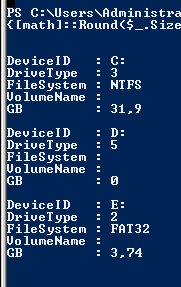
\includegraphics[width=0.3\textwidth]{Recursos/usb_estado_inicial.png}
\caption{Estado inicial del dispositivo: unidad \cod{E:} extraíble en FAT32.}
\label{fig:usb-inicial}
\end{figure}

\begin{figure}[H]
\centering
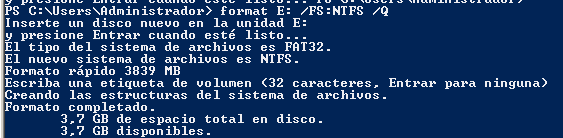
\includegraphics[width=0.8\textwidth]{Recursos/usb_formato_ntfs.png}
\caption{Formato rápido de la unidad \cod{E:} en NTFS.}
\label{fig:usb-formato}
\end{figure}

\begin{figure}[H]
\centering
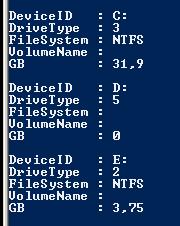
\includegraphics[width=0.3\textwidth]{Recursos/usb_estado_final.png}
\caption{Estado final del dispositivo: unidad \cod{E:} en NTFS.}
\label{fig:usb-final}
\end{figure}

\subsubsection{Simulación de la fuga}
La fuga se simuló desde la propia máquina virtual el jueves 12 de noviembre de
2026 (hora de la máquina virtual), siguiendo estos pasos:

\begin{enumerate}
  \item A las 16:19:56 se copió \cod{Confidencial.pdf} desde
        \cod{C:\Empresa\ConfidencialInfo} a la unidad \cod{E:} del dispositivo
        USB (figura~\ref{fig:usb-copia}).
  \item Se comprobó que la copia era idéntica al original: su huella SHA-256
        coincide con la calculada previamente
        (figura~\ref{fig:usb-hash-copia}).
  \item A las 16:21:25 se borró el fichero del USB con \cod{Remove-Item}. Al
        tratarse de un dispositivo extraíble, que no dispone de papelera de
        reciclaje, el borrado es directo (figura~\ref{fig:usb-borrado}).
  \item A las 16:22:43 se expulsó el dispositivo mediante la opción <<Quitar
        hardware de forma segura>> y se desconectó de la máquina virtual.
\end{enumerate}

\begin{figure}[H]
\centering
\includegraphics[width=0.8\textwidth]{usb_copia.png}
\caption{Copia de \cod{Confidencial.pdf} al USB (16:19:56).}
\label{fig:usb-copia}
\end{figure}

\begin{figure}[H]
\centering
\includegraphics[width=0.8\textwidth]{usb_hash_copia.png}
\caption{Verificación de la huella SHA-256 de la copia en el USB.}
\label{fig:usb-hash-copia}
\end{figure}

\begin{figure}[H]
\centering
\includegraphics[width=0.8\textwidth]{usb_borrado.png}
\caption{Borrado del fichero del USB (16:21:25).}
\label{fig:usb-borrado}
\end{figure}

% ---------------------------------------------------------------------
\subsection{Cadena de custodia}
\label{sec:usb-custodia}
El dispositivo fue adquirido por el grupo con anterioridad a la simulación y no
había sido utilizado. Tras la simulación de la fuga (12 de noviembre de 2026)
permaneció guardado en una caja en el domicilio de uno de los integrantes hasta
el día de la adquisición. Durante ese periodo no se calculó ningún
\textit{hash} ni se precintó el soporte, por lo que el estado del dispositivo
queda fijado por el \textit{hash} obtenido en el momento de la adquisición
forense. Conforme al supuesto del enunciado, el director de la empresa, Jaime
Diez Zurro, entrega el soporte al grupo el día de la adquisición.

\begin{table}[H]
\centering
\small
\renewcommand{\arraystretch}{1.3}
\begin{tabular}{@{}p{0.22\textwidth}p{0.11\textwidth}p{0.13\textwidth}p{0.45\textwidth}@{}}
\toprule
\textbf{Fecha y hora} & \textbf{Entrega} & \textbf{Recibe} & \textbf{Motivo y observaciones} \\
\midrule
Anterior al 12/11/2026 (sin fecha exacta) & Comercio & Pablo &
Compra del pendrive \textit{General UDisk} de 3,75 GB. Sin uso previo;
formateado de fábrica en FAT32 con MBR. \\
12/11/2026, 16:09:56 & -- & Pablo &
Formato rápido a NTFS en la máquina virtual (hora tomada de los metadatos
NTFS del volumen). \\
12/11/2026, 16:19:56 a 16:22:43 & -- & Pablo &
Conectado a la máquina virtual: copia (16:19:56), borrado (16:21:25) y
expulsión (16:22:43) de \cod{Confidencial.pdf}. Las horas de borrado y
expulsión proceden del registro de la simulación. \\
12/11/2026, 16:22:43 a 20/11/2026 & -- & Pablo &
Guardado en una caja, en el domicilio de Pablo, sin precinto ni
\textit{hash} previo. \\
20/11/2026, 16:30 & Jaime Diez Zurro (supuesto) & Pablo &
Entrega del soporte al grupo para el peritaje, según el supuesto del
enunciado. Entrega simulada: el soporte ya obraba en poder de Pablo. \\
20/11/2026, 19:52 & Pablo & Pablo (perito) &
Conexión al equipo de análisis con protección contra escritura y cálculo del
primer \textit{hash}. \\
20/11/2026, 20:10 & Pablo (perito) & Pablo &
Soporte expulsado del equipo de análisis tras la adquisición y la
verificación. Queda en custodia de Pablo; el análisis se realiza sobre la copia
de trabajo. \\
\bottomrule
\end{tabular}
\caption{Registro de custodia del dispositivo USB.}
\label{tab:usb-custodia}
\end{table}

% ---------------------------------------------------------------------
\subsection{Adquisición de la evidencia}
\label{sec:usb-adquisicion}

\subsubsection{Protección contra escritura}
La adquisición se realizó el 20 de noviembre de 2026 desde un equipo con
\textit{Windows} 10 Pro (compilación 19045). Antes de conectar el soporte se
activó el bloqueo de escritura de los dispositivos de almacenamiento USB del
sistema, creando el valor \cod{WriteProtect} (DWORD) con valor 1 en la clave
\cod{HKLM\SYSTEM\CurrentControlSet\Control\StorageDevicePolicies}
(figura~\ref{fig:usb-writeprotect}).

\begin{figure}[H]
\centering
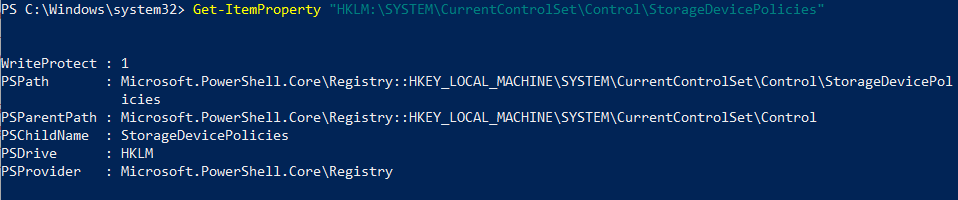
\includegraphics[width=0.9\textwidth]{Recursos/usb_writeprotect_registro.png}
\caption{Valor \cod{WriteProtect = 1} en el registro del equipo de análisis.}
\label{fig:usb-writeprotect}
\end{figure}

A las 19:52 se conectó el dispositivo. El sistema lo identificó como
\textit{General UDisk}, con el número de serie
\cod{2504021555480511776507}, tamaño de 4.026.531.840 bytes, tabla de
particiones MBR y la propiedad \cod{IsReadOnly} en \cod{True}, lo que confirma
que el soporte quedó montado en solo lectura (figura~\ref{fig:usb-getdisk}).

\begin{figure}[H]
\centering
\includegraphics[width=0.8\textwidth]{usb_get_disk.png}
\caption{Comprobación con \cod{Get-Disk}: el dispositivo figura como solo lectura.}
\label{fig:usb-getdisk}
\end{figure}

\subsubsection{Imagen forense en formato RAW}
Para la adquisición se utilizó \textit{Exterro FTK Imager} versión 8.3.0.27
(figura~\ref{fig:usb-ftk-version}), que permite acceder al disco físico sin
montarlo para escritura. Se adquirió la unidad física completa (no solo el
volumen) en formato RAW (dd), sin compresión ni cifrado y en un único segmento
(figura~\ref{fig:usb-ftk-destino}). Los datos del caso introducidos fueron:
número de caso \cod{ITP26-GP08}, número de evidencia \cod{USB-01} y la
descripción del soporte.

\begin{figure}[H]
\centering
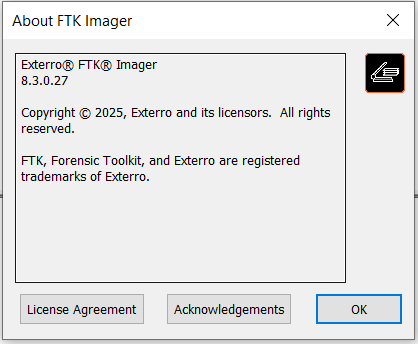
\includegraphics[width=0.3\textwidth]{Recursos/usb_ftk_version.png}
\caption{Versión de la herramienta de adquisición.}
\label{fig:usb-ftk-version}
\end{figure}

\begin{figure}[H]
\centering
\includegraphics[width=0.55\textwidth]{usb_ftk_destino.png}
\caption{Destino de la imagen: \cod{C:\Evidencias\USB\usb_evidencia}, sin
fragmentar.}
\label{fig:usb-ftk-destino}
\end{figure}

\begin{table}[H]
\centering
\small
\renewcommand{\arraystretch}{1.3}
\begin{tabular}{@{}p{0.34\textwidth}p{0.62\textwidth}@{}}
\toprule
\textbf{Parámetro} & \textbf{Valor} \\
\midrule
Fichero de imagen & \cod{usb_evidencia.001} \\
Formato & RAW (dd), un único segmento \\
Tamaño & 7.864.320 sectores de 512 bytes (4.026.531.840 bytes) \\
Inicio de la adquisición & 20/11/2026, 19:59:53 \\
Fin de la adquisición & 20/11/2026, 20:01:45 \\
Verificación & 20/11/2026, de 20:01:45 a 20:01:53 \\
\bottomrule
\end{tabular}
\caption{Parámetros de la adquisición.}
\label{tab:usb-adquisicion}
\end{table}

\subsubsection{Verificación de integridad}
Al terminar, la propia herramienta verificó la imagen y los \textit{hash} MD5
y SHA-1 recalculados coinciden con los obtenidos sobre el dispositivo original
durante la adquisición, sin bloques defectuosos
(figura~\ref{fig:usb-ftk-verif}). A continuación se calculó el SHA-256 de la
imagen con \cod{Get-FileHash} (20/11/2026, 20:02:51) y se creó la copia de
trabajo \cod{usb_trabajo.dd}, cuyo SHA-256 es idéntico al de la imagen.

\begin{figure}[H]
\centering
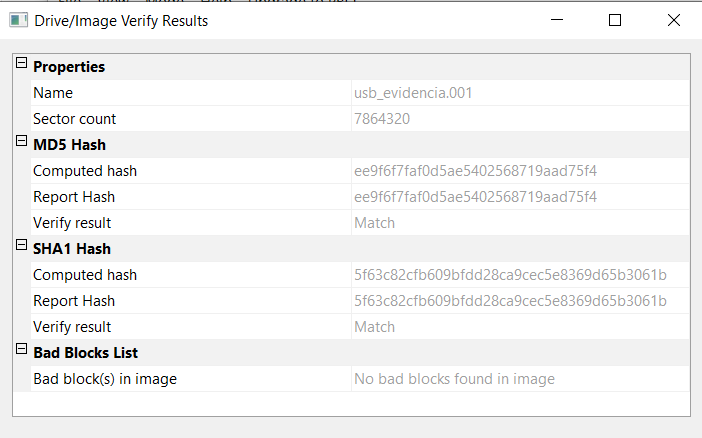
\includegraphics[width=0.7\textwidth]{Recursos/usb_ftk_verificacion.png}
\caption{Resultado de la verificación de la imagen: los \textit{hash} coinciden.}
\label{fig:usb-ftk-verif}
\end{figure}

\begin{table}[H]
\centering
\footnotesize
\renewcommand{\arraystretch}{1.3}
\begin{tabular}{@{}p{0.23\textwidth}p{0.11\textwidth}p{0.58\textwidth}@{}}
\toprule
\textbf{Elemento} & \textbf{Algoritmo} & \textbf{Hash} \\
\midrule
Dispositivo original & MD5 & \cod{ee9f6f7faf0d5ae5402568719aad75f4} \\
Dispositivo original & SHA-1 & \cod{5f63c82cfb609bfdd28ca9cec5e8369d65b3061b} \\
Imagen RAW & MD5 & \cod{ee9f6f7faf0d5ae5402568719aad75f4} \\
Imagen RAW & SHA-1 & \cod{5f63c82cfb609bfdd28ca9cec5e8369d65b3061b} \\
Imagen RAW & SHA-256 & \cod{53FC0DA61D1A733F8D4F1BDAB0A404CC}\newline
\cod{5306E040ABF46D5EEA8431F51FEAAC06} \\
Copia de trabajo & SHA-256 & \cod{53FC0DA61D1A733F8D4F1BDAB0A404CC}\newline
\cod{5306E040ABF46D5EEA8431F51FEAAC06} \\
\bottomrule
\end{tabular}
\caption{Verificación de integridad de la adquisición.}
\label{tab:usb-hashes}
\end{table}

\noindent\textbf{Importante.} Todo el análisis se realiza sobre la
\textbf{copia de trabajo}. La imagen original se conserva sin modificar, con
su \textit{hash} registrado en la cadena de custodia.

% ---------------------------------------------------------------------
\subsection{Análisis de la imagen}
\label{sec:usb-analisis}

El análisis se realizó con \textit{Autopsy} 4.23.1, sobre la copia de trabajo
\cod{usb_trabajo.dd}, que se añadió a un caso nuevo como fuente de datos de tipo
imagen de disco. Las horas que muestra la herramienta están en CET.

\subsubsection{Estructura del soporte}
La imagen contiene una tabla de particiones MBR con 7.864.320 sectores. Los
sectores 0 a 63 quedan sin asignar y el resto, del sector 64 al 7.864.319,
forma una única partición NTFS (tipo \cod{0x07}). Dentro del volumen solo
aparecen los ficheros propios del sistema de ficheros (\cod{\$MFT},
\cod{\$LogFile}, \cod{\$Extend}, etc.) y el fichero de usuario que se analiza
más adelante (figuras~\ref{fig:usb-autopsy-estructura} y
\ref{fig:usb-autopsy-volumen}). Los ficheros de sistema comparten la fecha
12/11/2026 16:09:56, que corresponde a la creación del volumen al darle formato
NTFS.

\begin{figure}[H]
\centering
\includegraphics[width=0.45\textwidth]{usb_autopsy_estructura.png}
\caption{Estructura del soporte en \textit{Autopsy}: espacio sin asignar y
partición NTFS.}
\label{fig:usb-autopsy-estructura}
\end{figure}

\begin{figure}[H]
\centering
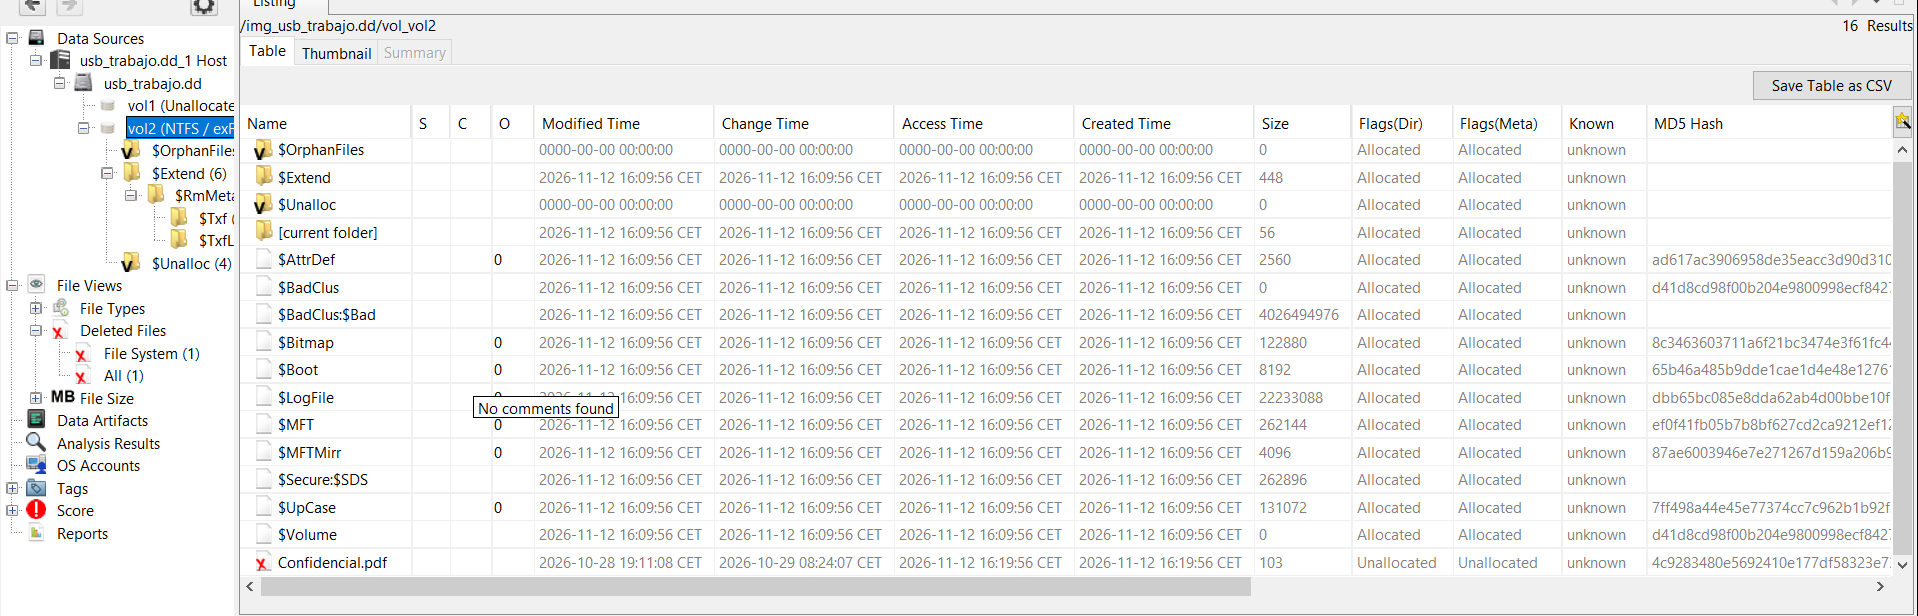
\includegraphics[width=\textwidth]{Recursos/usb_autopsy_volumen.png}
\caption{Contenido del volumen: ficheros de sistema NTFS y
\cod{Confidencial.pdf} sin asignar.}
\label{fig:usb-autopsy-volumen}
\end{figure}

\subsubsection{Localización del fichero borrado}
En el apartado \textit{Deleted Files} de la herramienta aparece una única
entrada, \cod{Confidencial.pdf}, que es además el único fichero de usuario del
volumen (figura~\ref{fig:usb-autopsy-borrado}). Está marcado como no asignado
tanto en el nombre como en los metadatos, y su tamaño es de 103 bytes, igual
que el del original.

\begin{figure}[H]
\centering
\includegraphics[width=\textwidth]{usb_autopsy_borrado.png}
\caption{Fichero borrado localizado en \textit{Deleted Files}.}
\label{fig:usb-autopsy-borrado}
\end{figure}

Sus metadatos (figuras~\ref{fig:usb-autopsy-meta1} y
\ref{fig:usb-autopsy-meta2}) indican que se trata de la entrada 35 de la
\cod{\$MFT}, no asignada, con dos nombres: el corto \cod{CONFID~1.PDF} y
\cod{Confidencial.pdf}.

\begin{figure}[H]
\centering
\includegraphics[width=0.6\textwidth]{usb_autopsy_metadatos1.png}
\caption{Metadatos del fichero en \textit{Autopsy}.}
\label{fig:usb-autopsy-meta1}
\end{figure}

\begin{figure}[H]
\centering
\includegraphics[width=0.6\textwidth]{usb_autopsy_metadatos2.png}
\caption{Atributos \cod{$STANDARD_INFORMATION} y \cod{$FILE_NAME} de la entrada
de la MFT.}
\label{fig:usb-autopsy-meta2}
\end{figure}

\subsubsection{Recuperación y comparación con el original}
El contenido del fichero se guarda dentro de la propia entrada de la MFT
(atributo \cod{$DATA} residente de 103 bytes,
figura~\ref{fig:usb-autopsy-data}). Por eso no fue necesario recurrir a
técnicas de \textit{carving} por firma: además, el fichero no es un PDF real,
sino un texto breve con extensión \cod{.pdf}, por lo que no tiene cabecera
\cod{\%PDF}. Se extrajo desde \textit{Autopsy} a la carpeta
\cod{C:\Evidencias\Recuperado} y se calculó su SHA-256, que coincide con el del
original (tabla~\ref{tab:usb-comparacion}). El contenido se muestra en la
figura~\ref{fig:usb-autopsy-hex}.

\begin{figure}[H]
\centering
\includegraphics[width=0.6\textwidth]{usb_autopsy_data_residente.png}
\caption{Atributo \cod{$DATA} residente, de 103 bytes.}
\label{fig:usb-autopsy-data}
\end{figure}

\begin{figure}[H]
\centering
\includegraphics[width=0.75\textwidth]{usb_autopsy_hex.png}
\caption{Contenido del fichero recuperado.}
\label{fig:usb-autopsy-hex}
\end{figure}

\begin{table}[H]
\centering
\footnotesize
\renewcommand{\arraystretch}{1.3}
\begin{tabular}{@{}p{0.30\textwidth}p{0.60\textwidth}@{}}
\toprule
\textbf{Fichero} & \textbf{SHA-256} \\
\midrule
Original (servidor) & \cod{f3ff86db9d526b85bab2afaf03722c32}\newline
\cod{1392f8b8dcae558d583704d713ef3fa7} \\
Recuperado del USB & \cod{F3FF86DB9D526B85BAB2AFAF03722C32}\newline
\cod{1392F8B8DCAE558D583704D713EF3FA7} \\
\bottomrule
\end{tabular}
\caption{Comparación del fichero recuperado con el original. Coinciden.}
\label{tab:usb-comparacion}
\end{table}

\subsubsection{Línea temporal}
La tabla~\ref{tab:usb-linea} reúne los hechos de la simulación. Las dos
primeras fechas se obtienen de los metadatos del sistema de ficheros; el
sistema de ficheros no guarda la hora del borrado ni la de la expulsión, por lo
que esas dos horas proceden del registro de la simulación.

\begin{table}[H]
\centering
\small
\renewcommand{\arraystretch}{1.3}
\begin{tabular}{@{}p{0.24\textwidth}p{0.40\textwidth}p{0.28\textwidth}@{}}
\toprule
\textbf{Fecha y hora} & \textbf{Hecho} & \textbf{Fuente} \\
\midrule
12/11/2026, 16:09:56 & Creación del volumen NTFS & Metadatos NTFS \\
12/11/2026, 16:19:56 & Copia de \cod{Confidencial.pdf} al USB & Fechas de creación y acceso \\
12/11/2026, 16:21:25 & Borrado del fichero & Registro de la simulación \\
12/11/2026, 16:22:43 & Expulsión del dispositivo & Registro de la simulación \\
\bottomrule
\end{tabular}
\caption{Línea temporal de la fuga.}
\label{tab:usb-linea}
\end{table}

Los atributos \cod{$FILE_NAME} del fichero muestran 12/11/2026 16:19:56 en
todas sus fechas, que es el momento de la copia. En \cod{$STANDARD_INFORMATION},
la fecha de creación y la de acceso coinciden con ese mismo instante, la de
modificación conserva la del original (28/10/2026, 19:11:08) y la de
modificación de la entrada (\textit{MFT Modified}) es 29/10/2026, 08:24:07,
anterior a la copia. No se ha podido comprobar el origen de esta última fecha;
una explicación posible es que se haya trasladado desde el fichero original al
copiarlo, aunque esto es solo una hipótesis. La salida de \cod{istat} muestra
las mismas fechas con una hora de diferencia por la zona horaria con la que las
presenta; en este informe se utilizan las de la tabla de \textit{Autopsy}, que
coinciden con las del original en la máquina virtual.

% ---------------------------------------------------------------------
\subsection{Conclusiones}
El fichero \cod{Confidencial.pdf} se ha recuperado completo del dispositivo
USB a pesar de haber sido borrado. Se encontraba en una entrada no asignada de
la MFT, con su contenido residente, y su SHA-256 coincide con el del fichero
original, por lo que es idéntico a este. La imagen se adquirió en formato RAW
con protección contra escritura, y el análisis se realizó sobre una copia de
trabajo con el mismo \textit{hash}.

Las limitaciones son las siguientes. El sistema de ficheros no conserva la hora
del borrado, por lo que no se puede acreditar a partir del soporte quién lo
realizó ni cuándo. Además, el soporte estuvo sin precinto ni \textit{hash}
desde el 12 de noviembre de 2026 hasta el día de la adquisición, de modo que su
estado queda fijado desde ese momento. Por último, la fecha \textit{MFT
Modified} de \cod{$STANDARD_INFORMATION} no se ha podido explicar con
certeza.
